\begin{comment}
\end{comment}

\chapter{Circuits pour la tolérance aux fautes quantique}

Pour terminer le récit de ma thèse,
j'enrichis le modèle de correction d'erreurs quantique
du chapitre précédent pour présenter la conception d'une mémoire quantique.
Il s'agit d'un système quantique permettant de stocker
de l'information pour une durée indéterminée.
Cependant,
comme mentionné au chapitre précédent,
les systèmes quantiques sont sujets aux erreurs,
même lorsqu'aucune opération n'est effectuée.
Ainsi,
pour construire une mémoire quantique,
il est nécessaire, encore une fois,
d'utiliser un code correcteur pour corriger les erreurs au fur et à mesure
qu'elles affectent le système.
Du moins,
il faut s'assurer que les erreurs restent assez faibles afin de pouvoir utiliser
l'information stockée dans le système pour un calcul futur.

En principe,
il est possible d'utiliser n'importe quel code correcteur pour construire
une mémoire quantique,
mais certains ont des propriétés plus favorables.
D'abord,
il est difficile de mettre à l'échelle un code correcteur dont le graphe
de Tanner est local, c'est-à-dire un graphe où la distance entre chaque paire de sommets 
connectés par une arête est bornée indépendamment du nombre de sommets.
Plus précisément,
Bravyi, Poulin et Terhal~\cite{bravyi_tradeoffs_2010}
ont montré que pour un tel code $[n, k]$,
la distance minimale $d$ est limitée par
\begin{equation}
	d^2 \leq c \frac{n}{k},
\end{equation}
pour une constante $c$ indépendante de $n$, $k$ et $d$.
Ainsi,
si $k$ augmente proportionnellement avec $n$,
la distance minimale est bornée par une constante.
De plus,
pour avoir une distance minimale raisonnable,
le nombre de qubits encodés $k$ 
ne doit pas, ou très peu, augmenter avec $n$.

Ce résultat implique que pour un grand $n$,
soit peu de qubits sont encodés,
soit ces derniers sont mal protégés des erreurs.
Il est donc difficile d'utiliser ces codes pour construire une mémoire 
quantique de grande taille.
Cependant,
lorsque la contrainte de localité du graphe de Tanner est levée,
Gottesman~\cite{gottesman_fault-tolerant_2013} a montré qu'il est possible 
de construire une mémoire quantique protégeant efficacement des erreurs,
avec $\frac{k}{n}$ constant, en utilisant des codes LDPC.
Conséquemment,
il est possible d'utiliser des codes LDPC pour construire 
des mémoires quantiques à grandes échelles.

D'un point de vue expérimental,
les codes LDPC ont l'avantage de pouvoir être implémentés de sorte que 
chaque qubit soit connecté à un nombre borné d'autres qubits.
Comme je le présenterai plus tard lorsque j'introduirai les circuits
de mesures de syndromes,
cela permet d'implémenter efficacement les circuits nécessaires à la
construction d'une mémoire quantique,
à la condition de pouvoir coupler n'importe quelle paire de qubits 
indépendamment de la distance qui les sépare.

Comme les couplages à longue portée sont difficiles pour plusieurs technologies de qubits,
il est tentant d'essayer d'implémenter des codes dont le graphe de Tanner est non local
à l'aide d'une architecture de qubits interagissant localement,
quitte à payer un léger surcout, c'est-à-dire utiliser des qubits supplémentaires
pour compenser le manque de connectivité.
Cependant,
dans un article qui n'est pas présenté dans cette thèse~\cite{delfosse_bounds_2021},
Nicolas Delfosse, Michael Beverland et moi-même avons montré que le cout de cette approche
est en réalité beaucoup trop élevé.
Plus précisément,
nous avons montré que pour implémenter une mémoire à l'aide d'un bon code LDPC
avec un rendement $k/n$ constant,
le nombre total de qubits nécessaires $N$ et la profondeur du circuit $\tau$ sont 
bornée inférieurement par 
\begin{align}
	N^{1/2} \tau \geq c n,
\end{align}
où $c$ est une constante.
Ainsi,
soit un très grand nombre de qubits sont nécessaires,
soit le circuit doit être très long.
Dans les deux cas,
augmenter ces quantités offre plus d'occasions aux erreurs de se manifester,
ce qui réduit significativement la qualité de la mémoire.

L'article présenté dans ce chapitre introduit une nouvelle architecture pour une mémoire quantique
qui permet d'implémenter des circuits pour de bons codes LDPC sans qu'il y ait de
croisement entre les couplages.
Bien que cela ne permette pas de régler le problème des couplages à longue portée,
il s'agit d'un premier pas dans la bonne direction puisque les croisements
entre les couplages sont une limitation importante aux connexions plus longues
pour plusieurs technologies de
qubits~\cite{sarovar_detecting_2020, debnath_demonstration_2016, neill_blueprint_2018, ash-saki_analysis_2020}.
Par exemple, 
les impressions de cuivre d'un circuit imprimé conventionnel ne peuvent pas se croiser
pour des raisons évidentes.
De plus,
l'approche utilisée repose sur des algorithmes de traçage de graphes,
régulièrement utilisés pour l'intégration à très grande échelle de composantes électroniques
sur des puces classiques~\cite{leighton_complexity_1983},
mais jusqu'alors peu ou pas utilisés pour le design de systèmes quantiques.
Comme des expériences numériques démontrent le potentiel de cette approche pour la réduction
des erreurs dans une mémoire quantique,
les travaux de cet article ouvrent la porte à utiliser davantage les méthodes 
de tracés de graphes pour la conception de systèmes quantiques.

Pour le reste de ce chapitre,
je présenterai d'abord les notions nécessaires de tolérance aux fautes et les modèles 
de bruits correspondant à une mémoire quantique.
Par la suite,
j'introduirai les codes de produit d'hypergraphes,
les codes LDPC utilisés dans les expériences numériques,
avant de présenter l'article.

\section{Tolérance aux fautes quantique}

\begin{figure}
	\begin{center}
		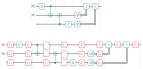
\includegraphics{figures/teleportation_bruit.pdf}
	\end{center}
	\caption{
		Versions idéale (haut) et bruitée (bas) du circuit de téléportation quantique.
	}
	\label{fig:teleportation_bruit}
\end{figure}

Dans un scénario idéal,
un circuit quantique est composé de transformations unitaires,
de préparations d'états, de mesures et de traitements classiques et toutes ces opérations
se font sans erreurs.
Par contre,
ce scénario,
bien que très utile pour concevoir des algorithmes quantiques,
est loin de la réalité où chaque opération est imparfaite.
Dans le modèle que je considère pour ce chapitre et les travaux associés,
ces imperfections dans les opérations sont représentées en ajoutant,
à la suite de chaque opération parfaite,
un canal bruité tel qu'illustré à la figure~\ref{fig:teleportation_bruit}.
De plus,
comme les circuits considérés incluent du traitement classique,
il est supposé que les bits sont parfaits,
ce qui est assez près de la réalité.

Selon l'opération qui est effectuée,
un canal bruité différent est utilisé.
Dans tous les cas,
la probabilité d'une erreur est $p$.
De plus, 
le circuit est divisé en étapes telles qu'à chacune d'elles,
exactement une opération affecte chaque qubit.
Pour ce faire,
lorsqu'un qubit est inactif,
l'opérateur $I$ est appliqué.
Également,
il n'est pas exclu qu'une opération affecte plusieurs qubits lors de la même étape.

Pour la préparation d'un état propre de $Z$, soit $\ket 0$ ou $\ket 1$,
le canal 
\begin{align}
\mathcal E_X(\rho) = (1 - p)\rho + pX\rho X
\end{align}
est appliqué.
Un canal similaire, $\mathcal E_Z$, est appliqué après la préparation
d'un état propre de $X$.
Ensuite,
le canal
\begin{align}
	\mathcal E_1(\rho) = (1 - p)\rho + \frac{p}{3}(X\rho X + Y\rho Y + Z\rho Z)
\end{align}
est appliqué après une transformation unitaire à un seul qubit.
Dans ce cas,
lorsqu'il y a une erreur,
celle-ci est choisie uniformément entre $X$, $Y$ et $Z$.
De même,
après une transformation unitaire à deux qubits,
le canal
\begin{align}
	\mathcal E_2(\rho)
	= (1 - p)\rho
	+ \frac{p}{15}\sum_{P \in \mathcal P_2^*\setminus \qty{II}} P\rho P
\end{align}
est appliqué,
où $\mathcal P_2^*$ est le groupe de Pauli à deux qubits sans les phases.
Finalement,
à la suite d'une mesure d'un opérateur de Pauli,
le résultat est renversé avec probabilité $p$.
Cela est équivalent au canal binaire symétrique du premier chapitre
et est noté $\mathcal E_m$.

Le circuit de téléportation illustré à la figure~\ref{fig:teleportation_bruit},
dans sa version idéale et sa version bruitée,
constitue dans son ensemble une transformation (non unitaire) à un qubit.
En effet,
bien que celui-ci comporte trois qubits,
seul le troisième peut avoir un état arbitraire en entrée et un seul qubit reste à la sortie.
L'ensemble des circuits que je considérerai ont cette forme,
c'est-à-dire qu'ils transforment $s$ qubits vers $s'$ qubits de manière 
potentiellement non unitaire à l'aide de diverses opérations classiques et quantiques
et de qubits supplémentaires.
Je noterai $N$ le nombre total de qubits du circuit et $\tau$
sa profondeur, soit le nombre d'étapes. 

En raison de l'ajout d'un canal bruité après chaque opération,
il est peu probable que l'état à la sortie du circuit soit l'état désiré.
Pour contrer ce problème,
les états à l'entrée et la sortie du circuit sont encodés dans un code correcteur.
Cela implique par contre de modifier le circuit pour prendre en compte l'encodage des qubits.
Pour évaluer la capacité d'un circuit modifié à tolérer les erreurs,
on vérifie si un décodeur idéal, comme le décodeur de maximum de vraisemblance, est en 
mesure de corriger les erreurs à la sortie du circuit~\cite{gottesman_introduction_2009}.
Ainsi,
pour un circuit $C$,
un état arbitraire $\ket{\psi}$,
sa version encodée $\ket{\bar{\psi}}$ à l'aide d'un code $[n, k]$
et un décodeur optimal $\mathcal D$,
un circuit $T$ est une adaptation tolérante aux fautes de $C$ si,
avec forte probabilité,
\begin{align}
	\mathcal D\qty(\mathcal E_T\qty(\op{\bar \psi}) )
	= \op{\bar \phi},
	\label{eq:tol_faute_condition}
\end{align}
où $\ket{\bar \phi}$ est la version encodée de $\ket{\phi} = C \ket\psi$
et $\mathcal E_T$ est obtenu en ajoutant une canal bruité après chaque opération
de $T$ comme à la figure~\ref{fig:teleportation_bruit}.

Il n'est pas évident qu'il est possible de construire des circuits tolérants aux fautes
puisque l'encodage demande d'utiliser un plus grand nombre de qubits,
ce qui représente un plus grand risque d'erreurs.
Par contre,
le théorème du seuil~\cite{aharonov_fault-tolerant_1999} stipule que si la probabilité d'erreur
par opération $p$ est inférieure à une valeur seuil $p^*$,
alors il est possible de construire un circuit tolérant aux fautes satisfaisant
l'équation~\ref{eq:tol_faute_condition} avec une probabilité arbitrairement près de 1.
La probabilité de seuil mesurée en pratique dépend des codes correcteurs utilisés
et des détails d'implémentation du circuit.
Ainsi,
la valeur de ce seuil est une métrique importante dans la performance d'un circuit tolérant aux fautes.
En effet,
un seuil élevé permet d'utiliser le circuit avec des systèmes plus bruyants.

Le cas étudié dans les travaux de cette thèse est le cas simple d'une mémoire quantique 
où la version idéale du circuit est composée uniquement de l'opérateur identité sur chaque qubit répété à chaque étape.
Bien que ce circuit semble très simple,
il s'agit d'un passage essentiel pour réaliser des circuits plus complexes comme le circuit
de téléportation.
De plus,
lorsque ce circuit est remplacé par sa version bruitée,
chaque qubit à chaque étape est affecté par le canal bruité $\mathcal E_1$.
Ainsi,
si rien n'est fait,
la probabilité d'avoir l'état initial après $t$ étapes pour $k$ qubits est de l'ordre de $p^{kt}$,
c'est-à-dire qu'elle diminue exponentiellement avec $k$ et $t$.

L'astuce pour construire une mémoire quantique tolérante aux fautes
est de constamment faire la correction des erreurs.
Ainsi,
le circuit est remplacé par une succession de mesures du syndrome
et d'application de la correction obtenue par un décodeur.
Bien sûr, 
chacune des opérations nécessaires dans les deux cas est suivie d'un canal bruité.

En général,
le décodeur n'est pas optimal puisque cela requiert un temps de calcul beaucoup trop élevé.
Il est plutôt commun de choisir un décodeur sous-optimal,
mais trouvant une correction en temps polynomial.
Dans ce cas,
on suppose que le temps de décodage est nul 
et qu'aucune erreur n'apparait lors du traitement classique.

Dans le cadre de cette thèse,
je ne m'intéresse pas aux décodeurs et je me contente des algorithmes de décodage standards.
Cela me permet de me concentrer sur les circuits de mesure du syndrome.
Dans le cas idéal,
un circuit de mesure du syndrome prend en entrée un état arbitraire et 
retourne une séquence de bits correspondant au syndrome de l'état résultant 
à la fin du circuit.
Il s'agit donc d'une mesure projective d'une superposition arbitraire
d'états de syndromes différents vers un sous-espace d'états de même syndrome.

Les mesures se font à l'aide d'opérations appartenant au groupe de Clifford,
de préparation des états propres de $X$ et $Z$ et de la mesure de ces opérateurs
pour un seul qubit.
Le groupe de Clifford est l'ensemble des transformations unitaires $U$ telles que,
pour tout opérateur de Pauli $P \in \mathcal P$,
il existe un $Q \in \mathcal P$ pour lequel $PU = UQ$.
Comme les erreurs sont décomposées sur la base des opérateurs de Pauli,
il est possible de remplacer une erreur appliquée avant un opérateur de Clifford
par une erreur appliquée après.
Cela permet ainsi de remplacer toutes les erreurs affectant un circuit composé d'opérateurs de Clifford,
par une seule erreur à la fin du circuit.

Le groupe de Clifford est généré par l'opérateur de Hadamard $H$,
l'opérateur de phase $S$ et l'opérateur de non-contrôlé $\text{CNOT}$
et inclut, entre autres, les opérateurs de Pauli.
Parmi ces opérateurs,
la porte $\text{CNOT}$,
inversant le deuxième qubit si le premier est dans l'état $\ket{1}$,
est l'unique opérateur utilisé pour la construction des circuits de mesure du syndrome 
présentés dans l'article.
L'action de CNOT est 
\begin{align}
	\text{CNOT} = \op{00}{00} + \op{01}{01} + \op{10}{11} + \op{11}{10}
\end{align}
et l'on vérifie facilement que
\begin{align}
	&XI \cdot \text{CNOT} = \text{CNOT} \cdot XX,
	&&ZI \cdot \text{CNOT} = \text{CNOT} \cdot ZI, \notag \\
	&IX \cdot \text{CNOT} = \text{CNOT} \cdot IX,
	&&IZ \cdot \text{CNOT} = \text{CNOT} \cdot ZZ,
	\label{eq:cnot_pauli}
\end{align}
les autres relations étant générées à partir de ces dernières.

\begin{figure}
	\centering
	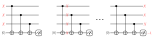
\includegraphics{figures/mesure_syndrome.pdf}
	\caption[Exemple de mesure de syndrome]{
		Propagation d'erreurs de type $X$ dans le circuit de mesure d'un
		stabilisateur de type $Z$ supporté sur trois qubits.
		L'erreur initiale, la conjugaison avec le premier CNOT 
		et l'état final en supposant un circuit idéal sont illustrés.
	}
	\label{fig:mesure_syndrome}
\end{figure}

Pour mesurer la parité d'un générateur du groupe stabilisateur de type $Z$,
un qubit supplémentaire, nommé qubit de mesure,
est d'abord préparé dans l'état $\ket 0$.
Ensuite,
une opération CNOT est faite à partir de chacun des qubits supportant le stabilisateur
vers le qubit de mesure.
Finalement,
ce qubit est mesuré dans la base de l'opérateur $Z$.
Tel que mentionné à l'équation~\ref{eq:cnot_pauli},
une erreur $X$ affectant le premier qubit du CNOT est remplacée
par une erreur $X$ sur ce même qubit et sur le qubit de mesure.
Dans le cas contraire,
une erreur $X$ sur le qubit de mesure ne se propage pas sur l'autre qubit 
impliqué dans le CNOT.
Ainsi,
comme illustré à la figure~\ref{fig:mesure_syndrome},
après l'application des portes CNOT,
le qubit de mesure se retrouve dans l'état $X^r\ket{0}$ où 
$r$ est le nombre de qubits affectés par une erreur $X$ à l'entrée du circuit.
Une mesure dans la base $Z$ permet donc de mesurer la parité de $r$.
Comme les erreurs $Z$ n'ont aucun impact sur la valeur de la mesure,
cela complète le circuit.

Pour mesurer la parité d'un stabilisateur de type $X$,
un circuit similaire est utilisé.
Dans celui-ci,
le qubit de mesure est préparé dans l'état $\ket +$ au lieu de l'état $\ket 0$,
l'orientation des portes CNOT est inversée
et la mesure se fait dans la base de l'opérateur $X$.
Encore une fois,
il est possible de valider ce circuit avec les relations de l'équation~\ref{eq:cnot_pauli}.

Le circuit pour mesurer la totalité du syndrome est obtenu 
en enchainant les circuits pour mesurer la parité de chacun des
générateurs du groupe stabilisateur.
De prime abord,
cette approche a deux problèmes majeurs.
Premièrement,
la profondeur du circuit total augmente linéairement avec le nombre 
de générateurs.
Deuxièmement,
comme chaque opération est bruitée,
il est possible que le syndrome mesuré ne correspondent pas à l'état à la sortie 
du circuit.

Les travaux de ce chapitre traitent de ces deux problèmes.
D'abord,
il est montré qu'il est possible d'effectuer des mesures de syndrome en parallèle
pour tous les codes CSS.
Cela permet de réduire la profondeur du circuit à une constante qui ne dépend que
du degré du graphe de Tanner,
soit le nombre d'arêtes du sommet avec le plus de connexions.
Ensuite,
des simulations numériques ont montré que même avec cette approche simple
de mesure du syndrome,
le seuil de tolérance aux fautes obtenu avec les codes de produit d'hypergraphes
est du même ordre de grandeur que les meilleurs seuils connus.
Ainsi,
remplacer les circuits de mesure de chaque générateur par des circuits
naturellement plus tolérants aux fautes ne peut qu'améliorer les résultats qui seront présentés.
Il s'agit d'ailleurs d'une avenue intéressante pour de futurs travaux de recherche.

Dans la prochaine section,
je vais introduire les codes de produit d'hypergraphes, 
la famille de codes LDPC qui a été étudiée plus en détail dans l'article.

\section{Codes de produit d'hypergraphes et codes expanseurs}

Les codes de produit d'hypergraphes introduits par Tillich et Zémor~\cite{tillich_quantum_2014}
figurent parmi les codes LDPC les plus étudiés~\cite{grospellier_combining_2020, grospellier_numerical_2018, leverrier_quantum_2015, kovalev_improved_2012, kovalev_numerical_2018}.
Une raison de cet intérêt est qu'ils permettent d'obtenir de bonnes performances 
avec un rendement $k/n$ constant tout en ayant une construction relativement simple.
En effet,
ces derniers sont obtenus par une partition des sommets du produit cartésien de
deux codes correcteurs classiques.
Ainsi,
dans cette section,
je présenterai d'abord un formalisme pour les codes correcteurs classiques
différent de celui présenté au chapitre~\ref{chap:codes_polaires},
avant d'utiliser ce formalisme pour introduire formellement les codes
de produit d'hypergraphes.

\subsection{Codes linéaires}

Un code correcteur classique $\code$ est linéaire si $\vb x + \vb y \in C$ 
pour tous $\vb x, \vb y \in \code$.
Ainsi,
pour un code linéaire encodant $k$ bits avec $n$ bits,
il existe une matrice $G \in \corpsfini{2}^{n \times k}$,
nommée matrice génératrice,
dont les colonnes forment une base de $\code$.
Le code est alors le sous-espace
\begin{align}
	\code(G) = \qty{
		G \vb x : \vb x \in \corpsfini{2}^k
	},
\end{align}
de dimension $k$.
Comme le choix de base pour $\code$ n'est pas unique,
il existe plusieurs choix pour $G$.

De manière comparable aux codes stabilisateurs,
la capacité d'un code linéaire à corriger les erreurs dépend de la distance minimale entre 
les mots codes,
\begin{align}
	d = \min_{\vb x, \vb x' \in \code} | \vb x + \vb x'| = \min_{\vb x \in \code \setminus \qty{\vb 0}} |\vb x|,
\end{align}
où $|\cdot|$ est la norme de Hamming, soit le nombre de 1 dans un vecteur.
La seconde égalité est obtenue par linéarité des mots codes.
Un décodeur optimal est alors en mesure de corriger toutes les erreurs dont la norme de Hamming
est inférieure à $d/2$.

Alternativement,
un code est défini à partir d'une matrice de parité, $H \in \corpsfini{2}^{(n - k) \times n}$.
Dans ce cas,
\begin{align}
	\code(H) = \qty{
		\vb x \in \corpsfini{2}^n : H \vb x = \vb 0
	}.
\end{align}
Il est possible que $H$ ait plus de $n - k$ rangées si certaines d'entre elles 
sont linéairement dépendantes, par contre je me limiterai au cas où $H$ est 
de plein rang, donc que le nombre de rangées est exactement $n - k$.

Alors que la matrice $G$ est utile pour l'encodage des messages en mots codes,
la matrice $H$ est plutôt utile pour la détection des erreurs et le décodage.
En effet,
la matrice de parité est comparable au groupe stabilisateur pour les codes quantiques.
En autre,
le syndrome d'un vecteur $\vb z \in \corpsfini{2}^n$ est le vecteur $\sigma(\vb z) = H\vb z$
et les mots codes sont les vecteurs de syndrome nul.
Ainsi, un syndrome non nul indique la présence d'erreurs.
Finalement, puisque $H (G\vb x) = \vb 0$ pour tous $\vb x \in \corpsfini{2}^k$,
les matrices $G$ et $H$ doivent respecter la condition $HG = 0$.

Un exemple de code linéaire est le code de Hamming, dont la matrice
de parité est 
\begin{align}
	H = \begin{pmatrix}
		0 & 0 & 0 & 1 & 1 & 1 & 1 \\
		0 & 1 & 1 & 0 & 0 & 1 & 1 \\
		1 & 0 & 1 & 0 & 1 & 0 & 1
	\end{pmatrix}
\end{align}
et la matrice génératrice est 
\begin{align}
	G^T = \begin{pmatrix}
		1 & 1 & 1 & 0 & 0 & 0 & 0 \\
		1 & 0 & 0 & 1 & 1 & 0 & 0 \\
		0 & 1 & 0 & 1 & 0 & 1 & 0 \\
		1 & 1 & 1 & 1 & 1 & 1 & 1.
	\end{pmatrix}
\end{align}
En calculant les $2^4 = 16$ combinaisons linéaires possibles des 
rangées de $G^T$,
l'on obtient une distance minimale de trois pour le code de Hamming.
Ainsi,
ce code permet de corriger toutes les erreurs de norme un.

Un décodeur optimal pour le code de Hamming découle directement de la valeur du syndrome.
En effet, pour un mot code $\vb x$ affecté de l'erreur $\vb e$,
le syndrome est 
\begin{align}
	\sigma(\vb x + \vb e) = H\vb x + H\vb e = H\vb e
\end{align}
puisque $H \vb x = \vb 0$ par définition du code.
Ainsi, le syndrome ne dépend que de l'erreur et non du mot code.
La matrice $H$ est construite telle que le syndrome d'une erreur $\vb e$ de norme un
correspond à la représentation en binaire du numéro de la colonne.
Par exemple,
le syndrome de $\vb e = \begin{pmatrix} 0 & 0 & 0 & 1 & 0 & 0 & 0 \end{pmatrix}^T$
est $\sigma(\vb e) = \begin{pmatrix} 1 & 0 & 0 \end{pmatrix}^T$,
ce qui correspond à la représentation binaire du nombre 4.
Cela permet ainsi d'identifier que l'erreur affecte le quatrième bit et 
il suffit de renverser ce dernier pour retrouver le mot code initial.

Le code de Hamming est un exemple particulier et un syndrome ne permet généralement
pas d'identifier aussi facilement une erreur.
Par contre,
les algorithmes de décodage des codes linéaires sortent du cadre de cette thèse.
Il est suffisant de considérer que les méthodes standards de propagation des 
croyances sont utilisées~\cite{richardson_modern_2008}.

Idéalement,
il est désirable que 
le rendement $k/n$ et la distance relative $d/n$ d'une famille de codes
soient bornés inférieurement.
Un résultat étonnant est qu'une matrice de parité avec une faible densité de 1
choisie aléatoirement répond à ces critères avec forte probabilité~\cite{sipser_expander_1996}.
Ce résultat repose sur une représentation graphique des codes linéaires sous forme de graphe de Tanner.

Comme au chapitre précédent,
le graphe de Tanner d'une matrice de parité $H$,
est le graphe biparti $T = (B \cup P, A)$
où les sommets $B = \qty{b_1, \ldots, b_n}$ correspondent aux $n$ bits
et les sommets $P = \qty{p_1, \ldots, p_{n - k}}$ aux $n - k$ rangées de la matrice de parité.
L'arête $\qty{b_i, p_j} \in A$ si et seulement si $H_{ji} = 1$.
Pour la suite de cette section,
je considère que les graphes sont $(\Delta_B, \Delta_P)$-réguliers,
c'est-à-dire que le degré de tous les sommets de $B$ ($P$) est $\Delta_B$ ($\Delta_P$).
Pour se limiter aux graphes de Tanner à faible densité,
$\Delta_B$ et $\Delta_P$ sont fixés indépendamment du nombre de qubits $n$.
Les codes considérés sont donc des codes LDPC.

Une mesure importante de la capacité d'un code à corriger les erreurs
est l'expansion du graphe du Tanner.
Un graphe biparti $G = (B\cup P, A)$, $(\Delta_B, \Delta_P)$-régulier,
est $(\alpha_B, \beta_B)$-expanseur à gauche si,
pour tout $S \subseteq B$ tel que $|S| \leq \alpha_B |B|$,
\begin{align}
	|\eta(S)| \geq (1 - \beta_B) \Delta_B |S|,
\end{align}
où $\eta(S)$ est l'ensemble des sommets dans le voisinage de $S$.
De même,
ce graphe est $(\alpha_P, \beta_P)$-expanseur à droite si,
pour tout $S \subseteq P$ tel que $|S| \leq \alpha_P |P|$,
\begin{align}
	|\eta(S)| \geq (1 - \beta_P) \Delta_P |S|.
\end{align}
Finalement,
le graphe est $(\alpha_B, \beta_B, \alpha_P, \beta_P)$-expanseur
s'il est $(\alpha_B, \beta_B)$-expanseur à gauche
et $(\alpha_P, \beta_P)$-expanseur à droite.

Comme $\Delta_B|S|$ est la cardinalité maximale du voisinage d'un
sous-ensemble $S \subseteq B$,
il suit qu'un graphe est expanseur à gauche si la cardinalité de 
chaque sous-ensemble de taille raisonnable est près de la valeur optimale.
Une intuition similaire s'applique aux différentes variations de l'expansion.
Ainsi,
un graphe expanseur est un graphe relativement bien connecté,
malgré une faible densité d'arêtes.

La propriété d'expansion est importante pour la correction d'erreurs puisqu'un code correcteur
avec un graphe de Tanner $(\Delta_B, \Delta_P)$-régulier et $(\alpha_B, \beta_B)$-expanseur à gauche,
avec $\beta_B > 1/2$,
possède une distance minimale d'au moins $\alpha_B n$~\cite{sipser_expander_1996}.
De plus,
avec forte probabilité lorsque $n$ augmente,
un graphe biparti régulier choisi aléatoirement est expanseur~\cite{sipser_expander_1996}.
En combinant ces deux résultats,
on conclut qu'avec forte probabilité,
un code choisi aléatoirement possède une distance minimale proportionnelle à $n$.
Également, comme $1 - \Delta_B / \Delta_P = k/n$,
il est possible de fixer les degrés pour obtenir un rendement arbitraire et constant.
Ainsi,
cette approche permet de générer une famille de codes avec $k \sim n$ et $d \sim n$,
ce qui est asymptotiquement optimal.

Dans la prochaine section,
j'aborderai comment utiliser une paire de graphes de Tanner expanseurs classiques
pour construire de bons codes correcteurs quantiques.
Cela complètera les notions nécessaires pour comprendre l'article du chapitre.

\subsection{Produit d'hypergraphes}

Au chapitre~\ref{chap:construction_codes},
j'ai présenté une méthode novatrice pour construire des codes CSS.
Pour les travaux de ce chapitre,
j'utilise plutôt une famille existante de codes CSS,
les codes de produit d'hypergraphes~\cite{tillich_quantum_2014}.

D'abord,
je rappelle qu'un code CSS est un code stabilisateur pour lequel les générateurs du groupe
stabilisateur se partitionnent en deux sous-groupes, 
les générateurs de type $X$ et les générateurs de type $Z$.
Ces sous-groupes sont respectivement représentés par les matrices de parité $H_X$ et $H_Z$.
Pour assurer que les stabilisateurs commutent,
la condition $H_X H_Z^T = 0$ est imposée.
Comme discuté au chapitre précédent,
il est difficile de construire une paire de codes linéaires
respectant cette condition.
Le produit d'hypergraphes est en fait une méthode pour construire
une telle paire de codes à partir d'une seconde paire de codes linéaires
ne respectant pas nécessairement la condition.

Le produit d'hypergraphes de deux codes linéaires $C_1$ et $C_2$
s'obtient à partir du produit cartésien des graphes de 
Tanner~\footnote{Le nom de \textit{produit d'hypergraphes} peut sembler étrange à première
vue puisque les graphes de Tanner sont des graphes bipartis. Cependant, les hypergraphes et les graphes
bipartis sont équivalents. Je me limite donc à la représentation par graphes bipartis.
Voir annexe~\ref{chap:theo_graphe}.} correspondants.
Le produit cartésien des graphes de Tanner $T_i = (B_i \cup P_i, A_i)$,
associés aux codes $C_i$, 
est le graphe 
\begin{align}
	T_1 \times T_2 = ((B_1 \cup P_1) \times (B_2 \cup P_2), A),
\end{align}
avec les arêtes 
\begin{align}
	A = 
	&\qty{
		\qty{(b_1, s_2), (p_1, s_2)} :
		\qty{b_1, p_1} \in A_1, s_2 \in B_2 \cup P_2
	} 
	\notag\\
	&\cup
	\qty{
		\qty{(s_1, b_2), (s_1, p_2)} :
		\qty{b_2, p_2} \in A_2, s_1 \in B_1 \cup P_1
	}.
\end{align}

\begin{figure}
	\centering
	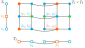
\includegraphics{figures/produit_hg.pdf}
	\caption[Produit d'hypergraphes]{
		Produit d'hypergraphes entre deux graphes de Tanner.
		Les sommets creux appartiennent aux graphes $T_1$ et $T_2$,
		alors que les sommets pleins sont ceux de $T_1 \times T_2$.
		Les ronds sont les sommets $Q = (B_1 \times B_2) \cup (P_1 \times P_2)$,
		les carrés sont les sommets $P_X = B_1 \times P_2$
		et les losanges sont les sommets $P_Z = P_1 \times B_2$.
		Les arêtes en gras ainsi que les sommets associés illustrent comment
		la contrainte d'orthogonalité est respectée.
	}
	\label{fig:produit_hg}
\end{figure}

Les sommets du produit cartésien $T_1 \times T_2$, 
se partitionnent en quatre ensembles:
$B_1 \times B_2$, $P_1 \times P_2$, $B_1 \times P_2$ et $P_1 \times B_2$.
Cette partition permet de construire les graphes de Tanner $T_X$ et $T_Z$.
Le graphe $T_X$ possède alors les sommets $B_X = B_1 \times B_2 \cup P_1 \times P_2$
et $P_X = B_1 \times P_2$.
De même,
le graphe de Tanner $T_Z$ possède les sommets $B_Z = B_X \equiv Q$
et $P_Z = P_1 \times B_2$.
Un exemple de produit d'hypergraphe est illustré à la figure~\ref{fig:produit_hg}.

Le produit d'hypergraphes assure l'orthogonalité de $H_X$ et $H_Z$.
En effet,
par définition du produit cartésien,
deux sommets $(b_1, p_2) \in P_X$ et $(p_1, b_2) \in P_Z$ 
ont comme uniques voisins communs potentiels les sommets $(b_1, b_2), (p_1, p_2) \in Q$.
Cela est le cas si $\qty{b_1, p_1} \in A_1$ et $\qty{b_2, p_2} \in A_2$.
Si ces deux conditions sont remplies,
les sommets $(b_1, p_2)$ et $(p_1, b_2)$ partagent deux voisins communs.
Sinon,
ils n'ont aucun voisin en commun.
Ainsi, le voisinage commun de chaque paire de sommets $(p_X, p_z) \in P_X \times P_Z$
contient soit deux ou zéro sommet de $Q$~\cite{tillich_quantum_2014}.
Cette contrainte,
qui implique l'orthogonalité de $H_X$ et $H_Z$,
est également illustrée à la figure~\ref{fig:produit_hg}.

Les matrices $H_X$ et $H_Z$ du produit d'hypergraphes des matrices
$H_1 \in \corpsfini{2}^{n_1 \times r_1}$
et
$H_2 \in \corpsfini{2}^{n_2 \times r_2}$
s'expriment directement selon~\cite{tillich_quantum_2014}
\begin{align}
	&H_X = (H_1 \otimes I_{n_2}\, \, \, I_{r_1} \otimes H_2^T),
	&H_Z = (I_{n_1} \otimes H_2 \, \, \, H_1^T \otimes I_{r_2}),
	\label{eq:prod_hg_mat}
\end{align}
où $(A \, \, \, B)$ est la concaténation des matrices $A$ et $B$.
Il est alors aisé de vérifier l'orthogonalité,
soit que
\begin{align}
	H_X H_Z^T 
	&=
	(H_1 \otimes I_{n_2})(I_{n_1} \otimes H_2)^T 
	+ (I_{r_1} \otimes H_2^T)(H_1^T \otimes I_{r_2})^T
	\notag \\
	&= 
	H_1 \otimes H_2^T + H_1 \otimes H_2^T
	\notag \\
	&= 0.
\end{align}
La dernière égalité se justifie du fait que $1 + 1 = 0$ pour le corps $\corpsfini{2}$.

Pour le reste de cette section,
je montrerai comment le produit d'hypergraphes permet de construire de bons codes CSS
à partir de codes classiques expanseurs.
Pour ce faire,
je me limiterai aux produits de codes $C_1 = C_2 \equiv C$ 
puisqu'il s'agit des codes utilisés dans l'article.
Ce résultat est présenté plus en détail par Leverrier et al~\cite{leverrier_quantum_2015}.

L'équation~\eqref{eq:prod_hg_mat} implique que les dimensions des matrices
$H_X \in \corpsfini{2}^{r_X \times n_q}$ et $H_Z \in \corpsfini{2}^{r_Z \times n_q}$ 
sont données par les paramètres $n_q = n_1 n_2 + r_1 r_2$, $r_X = r_1 n_2$ et $r_Z = n_1 r_2$.
Le code CSS correspondant possède ainsi $n_q$ qubits et $r_X + r_Z$ générateurs du groupe stabilisateur.
Le nombre de qubits encodés est alors
\begin{align}
	k_q 
	= 
	n_q - r_X - r_Z
	= (n_1 - r_1)(n_2 - r_2)
	= k_1 k_2.
\end{align}
Dans le cas où $n_1 = n_2 \equiv n$, $k_1 = k_2 \equiv k$ et $r_1 = r_2 \equiv r$,
les paramètres du code quantique sont $[n_q = n^2 + r^2, k_q = k^2]$.
Ainsi,
le code CSS résultant a un rendement $k_q / n_q$ constant lorsque le code linéaire utilisé 
a également un rendement $k/n$ constant.

La distance minimale $d_q$ d'un code CSS construit avec les codes linéaires $C_X$ et $C_Z$ 
ayant respectivement des distances minimales $d_X$ et $d_Z$ est~\cite{calderbank_good_1996}
\begin{align}
	d_q = \min(d_X, d_Z).
\end{align}
Cela découle du fait que pour des opérateurs $L_X$ et $L_Z$ respectivement de type $X$ et $Z$,
le poids du produit $L_X L_Z$ est au moins $\min(|L_X|, |L_Z|)$.

Lorsque $H_1 = H_2 \equiv H$,
l'équation~\eqref{eq:prod_hg_mat} devient
\begin{align}
	&H_X = (H \otimes I_{n}\, \, \, I_{r} \otimes H^T),
	&H_Z = (I_{n} \otimes H \, \, \, H^T \otimes I_{r}).
\end{align}
Ainsi,
$H_X(\vb x \otimes \vb u \, \, \, \vb 0) = \vb 0$ 
pour tous vecteurs $\vb x$ tels que $H \vb x = \vb 0$ et vecteurs $\vb u$ 
tels que $|\vb u| = 1$.
Dans ce cas,
$|(\vb x \otimes \vb u \, \, \, \vb 0)| = |\vb x|$.
Ainsi,
la distance minimale $d_X$ du code $C_X$ de matrice de parité $H_X$ est au moins la distance
minimale $d$ du code linéaire $C$.
De même,
il est possible de construire un vecteur orthogonal à $H_X$ à partir d'un vecteur $\vb x$
tel que $H^T \vb x = \vb 0$.
Ainsi,
\begin{align}
	d_X = \min(d, d^T),
\end{align}
où $d^T$ est la distance minimale du code de matrice de parité $H^T$.
Un argument similaire s'applique pour $d_Z$.
La distance minimale d'un code CSS est donc~\cite{tillich_quantum_2014}
\begin{align}
	d_q = \min(d_X, d_Z) = \min(d, d^T).
\end{align}

Comme montré à la section précédente,
un code linéaire $(\alpha_B, \beta_B, \alpha_P, \beta_P)$-expanseur a une
distance minimale $d \geq \alpha_B n$.
En transposant le graphe de Tanner associé,
on conclut que $d^T \geq \alpha_P r$.
Ainsi,
la distance minimale du produit d'hypergraphes d'un code expanseur est~\cite{leverrier_quantum_2015}
\begin{align}
	d_q \geq \min(\alpha_B n, \alpha_P r).
\end{align}
Cette approche permet ainsi de construire une famille de codes CSS tels que
$k_q \sim n_q$ et $d_q \sim \sqrt{n_q}$.
Puisque le nombre de qubits encodés et la distance minimale augmentent avec le nombre 
de qubits du code,
il est possible d'utiliser ces codes pour construire des systèmes tolérants aux fautes
avec un surcoût constant en qubits~\cite{gottesman_fault-tolerant_2013}.
Les travaux de l'article de ce chapitre avancent dans cette direction 
en introduisant une mémoire quantique tolérante aux fautes construite
à partir de codes de produit d'hypergraphes.

\section{Article}

L'article a été accepté et publié par la revue \textit{Physical Review Letters} à l'été 2022.

Dans celui-ci,
des circuits de mesure du syndrome de profondeurs constantes utilisables
pour tous les codes CSS LDPC sont présentés.
Au meilleur de ma connaissance,
il s'agissait alors de la première présentation concrète de tels circuits.
La construction de ces circuits repose sur un algorithme de coloration des
arêtes des graphes de Tanner.
De plus,
il est montré comment réduire davantage la profondeur du circuit pour les codes 
de produit d'hypergraphes.
Des mémoires quantiques sont simulées en utilisant ces circuits pour des 
produits d'hypergraphes de codes linéaires $(3, 4)$-réguliers.
Les résultats obtenus montrent clairement que l'utilisation de cette approche
réduit significativement le nombre de qubits nécessaires pour l'encodage
en comparaison aux codes de surfaces,
des codes très étudiés~\cite{kitaev_fault-tolerant_2003, dennis_topological_2002, fowler_surface_2012, fowler_high_2009, stephens_fault-tolerant_2014, bravyi_efficient_2014, darmawan_tensor-network_2017} 
où les graphes de Tanner sont limités à des connexions locales.

L'article introduit également une architecture multiplanaire pour implémenter une telle mémoire
en laboratoire.
Bien qu'il reste du travail à faire pour implémenter cette architecture
dans des conditions de laboratoire réelles,
la construction de cette dernière utilise une approche novatrice basée sur les algorithmes de traçage de
graphes.

J'ai effectué les travaux de cet article dans le cadre d'un stage 
dans l'équipe de Microsoft.
L'idée de voir le problème de construction de circuits de mesure du syndrome
comme un problème de coloriage de graphes a été proposée par mes superviseurs.
Par la suite,
j'ai poussé cette idée plus loin dans le cadre des produits d'hypergraphes.
De plus,
j'ai implémenté l'ensemble du logiciel de simulation en plus de faire les expériences numériques
et l'analyse des données.
J'ai également conçu l'architecture multiplanaire et effectué les preuves de l'article.
Finalement,
le travail de rédaction de l'article a été partagé également entre les trois auteurs.

Les travaux que j'ai effectués lors du stage ont également mené à une seconde 
publication~\cite{delfosse_bounds_2021},
qui n'est pas présentée dans cette thèse.

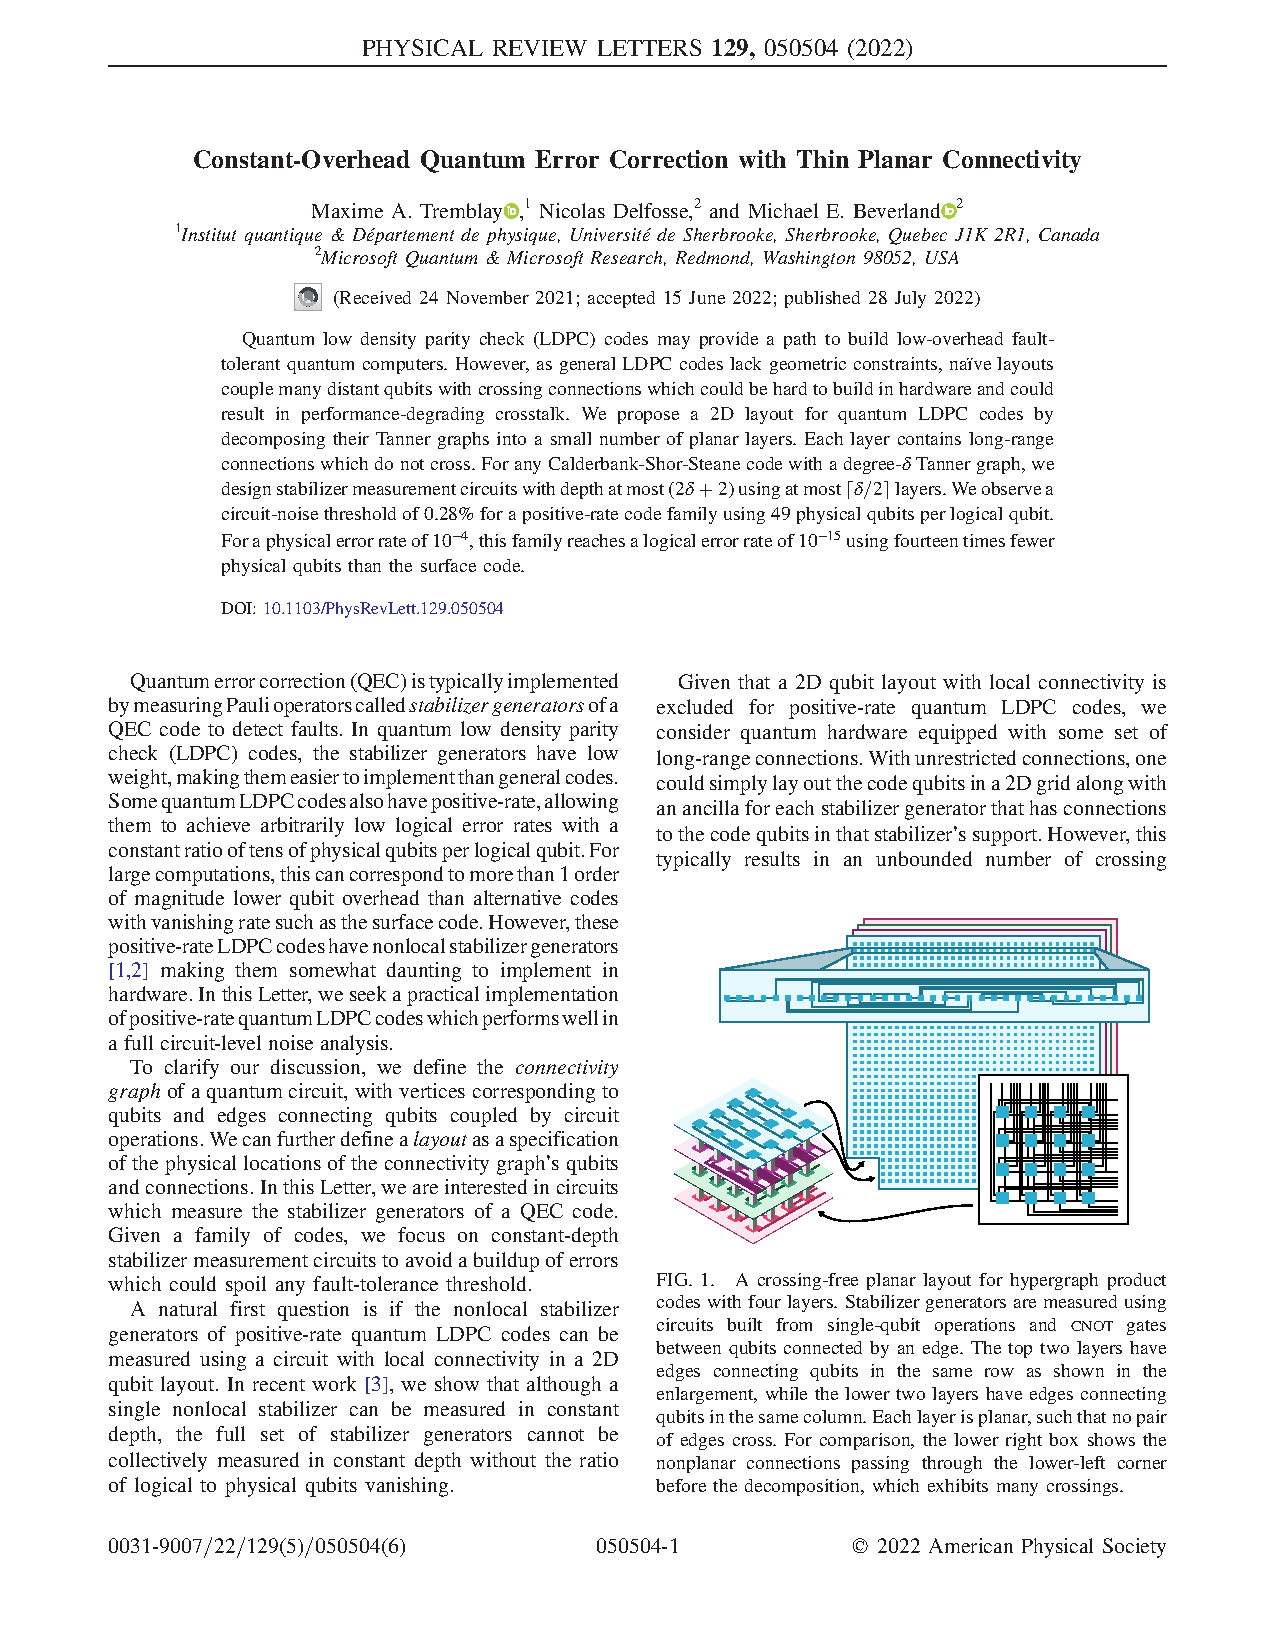
\includepdf[pages=-]{articles/planar_layout.pdf}

